% !TEX root = ../../main.tex
% File: part2/chapters1/chap1_5.tex

\section{Quản lý Dữ liệu và Phiên bản (Data Version Control - DVC)}
\label{sec:dvc}

Trong phát triển phần mềm truyền thống, **Git** là công cụ tiêu chuẩn để quản lý phiên bản của mã nguồn. Nó cho phép chúng ta theo dõi mọi thay đổi, quay lại các phiên bản cũ, và cộng tác một cách hiệu quả.

Tuy nhiên, trong các dự án học máy, \textbf{Mã nguồn chỉ là một phần của câu chuyện}. Kết quả của một mô hình không chỉ phụ thuộc vào code, mà còn phụ thuộc rất nhiều vào:
\begin{itemize}
    \item \textbf{Dữ liệu (Data):} Bộ dữ liệu nào đã được sử dụng để huấn luyện?
    \item \textbf{Mô hình (Model):} Trọng số của mô hình được tạo ra từ lần chạy nào?
    \item \textbf{Siêu tham số (Hyperparameters):} Các thiết lập như tốc độ học, kích thước batch là gì?
\end{itemize}

\begin{tcolorbox}[
    title=Vấn đề: "Nó chạy được trên máy của tôi mà!",
    colback=red!5!white, colframe=red!75!black, fonttitle=\bfseries
]
Nếu không có một hệ thống quản lý phiên bản hoàn chỉnh, chúng ta sẽ rơi vào một "địa ngục tái lập" (reproducibility hell). Bạn có thể có một mô hình hoạt động rất tốt, nhưng vài tháng sau, khi dữ liệu thay đổi hoặc một đồng nghiệp muốn tái tạo lại kết quả của bạn, không ai có thể làm được vì không ai biết chính xác phiên bản dữ liệu và các thiết lập nào đã tạo ra mô hình đó.
\end{tcolorbox}

\textbf{Git không được thiết kế để xử lý các file lớn} như các bộ dữ liệu hay các file trọng số mô hình. Việc commit các file lớn này sẽ làm cho kho Git trở nên cực kỳ cồng kềnh và chậm chạp. Đây là lúc DVC (Data Version Control) phát huy tác dụng.

\subsection{DVC là gì và Triết lý hoạt động}
\label{ssec:what_is_dvc}

\textbf{DVC} là một công cụ mã nguồn mở được thiết kế để mang lại khả năng quản lý phiên bản cho toàn bộ pipeline học máy. Nó hoạt động \textbf{bên trên Git}, không phải thay thế Git.

\begin{tcolorbox}[
    title=Triết lý của DVC,
    colback=blue!5!white, colframe=blue!75!black, fonttitle=\bfseries
]
Hãy để \textbf{Git} làm những gì nó giỏi nhất: quản lý phiên bản của các file code nhỏ. Hãy để một \textbf{bộ nhớ từ xa (remote storage)} (như Amazon S3, Google Cloud Storage, hoặc thậm chí là Google Drive) lưu trữ các file dữ liệu và mô hình lớn. \textbf{DVC} sẽ đóng vai trò là "cầu nối", tạo ra các file metadata nhỏ để theo dõi phiên bản của các file lớn đó, và các file metadata này sẽ được quản lý bởi \textbf{Git}.
\end{tcolorbox}

\subsubsection{Cơ chế hoạt động}
Khi bạn muốn theo dõi một file dữ liệu lớn (ví dụ: `data.csv`) bằng DVC, các bước sau sẽ xảy ra:
\begin{enumerate}
    \item \textbf{`dvc add data.csv`:}
        \begin{itemize}
            \item DVC sao chép file `data.csv` vào một thư mục ẩn gọi là `.dvc/cache`. Nội dung của file được lưu trữ dựa trên một giá trị băm (hash) duy nhất.
            \item DVC tạo ra một file metadata nhỏ, có tên là `data.csv.dvc`. File này chỉ chứa thông tin về file gốc, quan trọng nhất là giá trị băm của nó.
            \item DVC tự động thêm `data.csv` vào file `.gitignore` để Git sẽ bỏ qua file dữ liệu lớn này.
        \end{itemize}
    \item \textbf{`git add data.csv.dvc` và `git commit`:}
        \begin{itemize}
            \item Bây giờ, bạn sẽ commit cái file `data.csv.dvc` nhỏ xíu này vào Git.
            \item Bất kỳ ai clone kho Git của bạn sẽ có file metadata này.
        \end{itemize}
    \item \textbf{`dvc push`:}
        \begin{itemize}
            \item Lệnh này sẽ tải nội dung của file dữ liệu thực sự (từ `.dvc/cache`) lên bộ nhớ từ xa mà bạn đã cấu hình (ví dụ: một bucket S3).
        \end{itemize}
    \item \textbf{`dvc pull`:}
        \begin{itemize}
            \item Khi một đồng nghiệp clone kho Git, họ sẽ không có file `data.csv`. Nhưng họ có thể chạy lệnh `dvc pull`.
            \item DVC sẽ đọc file `data.csv.dvc`, tìm ra giá trị băm cần thiết, và tải về phiên bản dữ liệu chính xác từ bộ nhớ từ xa vào máy của họ.
        \end{itemize}
\end{enumerate}

\begin{center}
    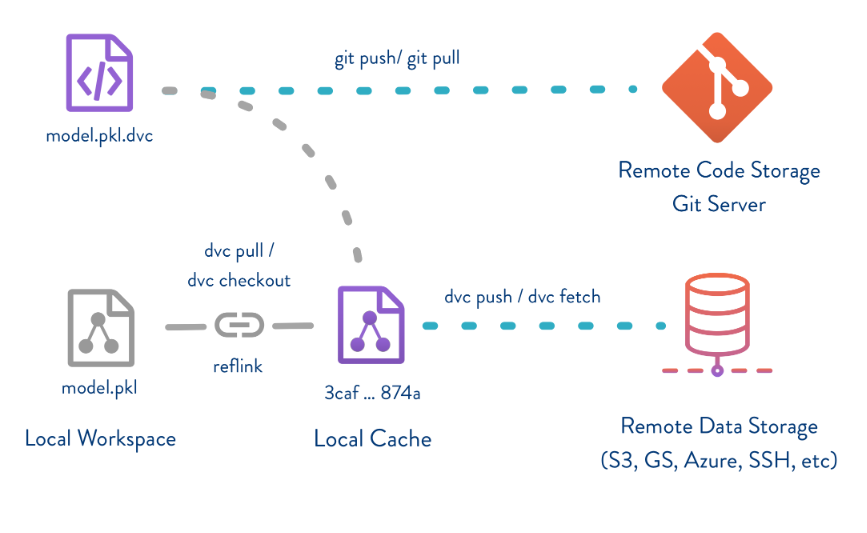
\includegraphics[width=1.0\textwidth]{images/dvc_workflowpng.png}
    \captionof{figure}{Luồng làm việc của DVC kết hợp với Git. Git quản lý code và các file metadata `.dvc`. DVC quản lý việc đồng bộ hóa các file dữ liệu/mô hình lớn với bộ nhớ từ xa.}
    \label{fig:dvc_workflow}
\end{center}

\subsection{DVC Pipelines: Tái lập toàn bộ Thử nghiệm}
\label{ssec:dvc_pipelines}
DVC còn tiến một bước xa hơn bằng cách cho phép bạn định nghĩa và kết nối các bước trong pipeline học máy của mình.

\begin{itemize}
    \item \textbf{Định nghĩa các Giai đoạn (Stages):} Bạn có thể tạo một file (ví dụ: `dvc.yaml`) để định nghĩa các giai đoạn của thử nghiệm, ví dụ: `preprocess`, `train`, `evaluate`.
    \item \textbf{Mô tả mỗi Giai đoạn:}
        \begin{itemize}
            \item \textbf{`cmd`:} Lệnh cần chạy (ví dụ: `python train.py`).
            \item \textbf{`deps` (Dependencies):} Các file đầu vào của giai đoạn này (ví dụ: code `train.py`, dữ liệu `data/train.csv`).
            \item \textbf{`outs` (Outputs):} Các file được tạo ra bởi giai đoạn này (ví dụ: file trọng số `model.pkl`, file metric `metrics.json`).
        \end{itemize}
    \item \textbf{Chạy và Tái tạo Pipeline (`dvc repro`):}
        \begin{itemize}
            \item Lệnh `dvc repro` (reproduce) sẽ tự động kiểm tra xem có bất kỳ file `deps` nào đã thay đổi hay không.
            \item Nếu có một sự thay đổi (ví dụ, bạn thay đổi một siêu tham số trong code hoặc cập nhật dữ liệu), DVC sẽ tự động chạy lại giai đoạn đó và tất cả các giai đoạn phụ thuộc vào nó.
            \item Nếu không có gì thay đổi, DVC sẽ không chạy lại, giúp tiết kiệm thời gian và tài nguyên tính toán.
        \end{itemize}
\end{itemize}
Bằng cách commit file `dvc.yaml` và `dvc.lock` (file ghi lại các giá trị băm chính xác của các deps/outs) vào Git, bạn đã ghi lại toàn bộ "provenance" (nguồn gốc) của một thử nghiệm. Bất kỳ ai cũng có thể checkout một commit Git cụ thể và chạy `dvc repro` để tái tạo lại chính xác kết quả của bạn.

\subsection{Lợi ích của việc sử dụng DVC}
\begin{itemize}
    \item \textbf{Tính tái lập (Reproducibility):} Đảm bảo rằng các thử nghiệm có thể được tái tạo một cách đáng tin cậy bởi bạn trong tương lai hoặc bởi các đồng nghiệp.
    \item \textbf{Cộng tác Dễ dàng:} Các thành viên trong nhóm có thể chia sẻ dữ liệu và mô hình một cách liền mạch mà không làm phình to kho Git.
    \item \textbf{Theo dõi Thử nghiệm:} DVC cho phép bạn so sánh các kết quả giữa các nhánh Git hoặc các commit khác nhau, giúp bạn hiểu rõ ảnh hưởng của các thay đổi (dữ liệu, code, siêu tham số) đến metric của mô hình.
    \item \textbf{Sự linh hoạt về Lưu trữ:} Hoạt động với nhiều loại backend lưu trữ khác nhau (S3, GCS, Azure Blob, HDFS, SSH, ...).
\end{itemize}
Việc tích hợp DVC vào quy trình làm việc đòi hỏi một chút nỗ lực ban đầu, nhưng lợi ích về lâu dài về sự ổn định, tính tái lập và khả năng cộng tác là vô giá trong bất kỳ dự án học máy nghiêm túc nào.

\bigskip
\hrule
\bigskip

\begin{center}
    \textbf{\Large KẾT THÚC CHƯƠNG 1}
\end{center}

\textit{Trong chương đầu tiên của phần thực chiến này, chúng ta đã xây dựng nền móng vững chắc cho bất kỳ dự án NLP thành công nào. Chúng ta đã bắt đầu với một quy trình làm việc có hệ thống, sau đó đi sâu vào công việc chiếm phần lớn thời gian và công sức: dữ liệu. Bạn đã học các kỹ thuật để thu thập, làm sạch, gán nhãn, tăng cường, và quan trọng là quản lý phiên bản dữ liệu một cách chuyên nghiệp. Bài học cốt lõi của chương này là: một pipeline dữ liệu mạnh mẽ và có thể tái lập chính là xương sống của một hệ thống AI hiệu năng cao. Giờ đây, khi đã có trong tay một bộ dữ liệu chất lượng, chúng ta đã sẵn sàng để chuyển sang giai đoạn hấp dẫn tiếp theo: huấn luyện và đánh giá các mô hình state-of-the-art.}